\section{Problem Solution}
\label{sec:solution}

Shown in Figure~\ref{fig:unfolded}, we show the regular pyramid of
Figure~\ref{fig:problem} unfolded onto the plane in such a manner that the edge
$OQ$ remains glued, while the edges $OR$, $OS$, and $OP$ are unglued. An
arbitrary piecewise straight path $\gamma$ from the vertex $P$ to the midpoint
$T$ is then depicted as the green curve on this figure. The continuous portions
of this path have lengths $\ell_1$ and $\ell_2$, respectively.

The line $PR$ that connects the vertices $P$ and $R$ is orthogonal to the edge
$OQ$ since the triangle $\triangle POQ$ is equilateral. Let the signed distance
from the intersection $M$ of $PR$ with $OQ$ to the intersection $U$ of our path
$\gamma$ and $OQ$ be given by $x$. In the following, we express the total length
$\ell_1 + \ell_2$ of our curve $\gamma$ as a function of this distance $x$ and
minimize it to arrive at the answer.

\begin{figure}[h]
  \centering
  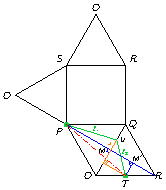
\includegraphics[trim={0 0 0
  0cm},clip,width=0.5\textwidth]{./figures/pyramid-unfolded.pdf}
  \vspace{-8mm}
  \caption{The unfolded regular pyramid.}
  \label{fig:unfolded}
\end{figure}

Since $PM \perp OM$, Pythagoras's theorem yields $\abs{PM} = \sqrt{3}\ell$. By
the same token, $\triangle PMU$ is a right triangle, yielding \[ \ell_1(x) =
\sqrt{x^2 + 3\ell^2}. \]
